\chapter{Entwicklung}

\section{Java Backend}

Im folgenden wird der Aufbau und die Funktionalität des Java Backends und der einzelnen Klassen dargestellt, auf Grund von Platzmangel wird hier nur auf die wichtigsten Funktionalitäten und Methoden eingegangen.

Die Klasse \enquote{Game} implementiert die Spiellogik und das Echtzeit-Konzept. Hier werden Aktionen, die alle Spieler beziehungsweise Unternehmen betreffen durchgeführt sowie die Unternehmen, beispielsweise für die Festlegung des Gewinners einer Ausschreibung, verglichen.

Die Hauptfunktionalität des Unternehmensplanspiels ist im Package \enquote{Unternehmung} umgesetzt, das, strukturell gesehen, \enquote{unter} der Klasse \enquote{Game} liegt. Hier sind neben der Klasse \enquote{Unternehmen} die einzelnen Abteilungen eines solchen mit ihren verschiedenen Möglichkeiten, die dem Spieler hier zur Verfügung stehen, implementiert (Package \enquote{Abteilungen}) sowie das Kennzahlenwesen eines Unternehmens (Package \enquote{Kennzahlen}). Darüber hinaus befinden sich in diesem Package die notwendigen Java-Klassen, durch deren Objekte ein objektorientierter Programmieransatz realisiert wird. Einige Methoden werfen Exceptions, die im Package \enquote{Exceptions} abgelegt sind.


\subsection{Die Klasse \enquote{Game}} \textnormal{\textsf{\small{Luca Dommes}}}}

In der Klasse Game ist die Logik und Mechanik des Untenehmensplanspiels implementiert, sie steht, strukturell gesehen, über allen anderen Klassen.

Zunächst einmal ist zu erwähnen, dass es sich hierbei um eine Spezialisierung der Java-Klasse \enquote{TimerTask}\footnote{https://docs.oracle.com/javase/8/docs/api/java/util/TimerTask.html} handelt. Dies dient der Umsetzung des Echtzeit-Ansatzes des Spiels. So wird im Konstruktor der Game-Klasse ein Timer-Objekt erstellt, das mit einem Intervall von 16 Minuten initialisiert wird. 16 Minuten stellen also einen Tag in Spielzeit dar. Im statischen Klassenattribut \enquote{gameCalendar} wird die Spielzeit als Calendar-Objekt\footnote{https://docs.oracle.com/javase/8/docs/api/java/util/Calendar.html} dargestellt, das bei jedem Timer Intervall einen Tag hochgezählt wird. Wenn 16 Minuten also ein Spieltag sind vergehen pro Stunde 3,75 Spieltage und dementsprechend an einem Tag (3,75 * 24 =) 90 Spieltage, sprich ein Quartal. Daraus folgt, dass ein Geschäftsjahr 4 (Echtzeit-)Tage dauert.

Die Klasse Game besteht hauptsächlich aus statischen Methoden, um die Zugriffe auf die Klasse zu erleichtern. Wie im Folgenden häufig beschrieben wird oftmals aus den verschiedensten Klassen auf die Klasse Game zugegriffen, unter Anderem um auf das Calendar-Objekt zuzugreifen und somit das aktuelle Datum abzugreifen. Hierfür müsste jeder Klasse das Game-Objekt mitgegeben werden. Durch die statischen Methoden wird dies überflüssig.

In der statischen ArrayList\footnote{https://docs.oracle.com/javase/8/docs/api/java/util/ArrayList.html} \enquote{companies} sind die Unternehmens-Objekte der einzelnen Mitspieler abgelegt. In einer zweiten ArrayList \enquote{companiesArchiv} werden Unternehmen im Falle des Bankrott abgelegt. Darüber hinaus gibt es noch eine ArrayList \enquote{\textbf{ausschreibungen}}, was es mit dieser Liste auf sich hat wird in \ref{Vertrieb} dargestellt.

In der statischen Map \enquote{highscores} werden die Spielstände gespeichert. Hier wird, entweder im Falle des Spielendes, also zehn Jahre nach Gründung eines Unternehmens, oder beim Bankrott eines Unternehmens, der Eigenkapital-Endbestand sowie der Unternehmensname abgespeichert. An das Frontend wird diese Liste über die Methode \enquote{getHighscoresAsTreeMap()} als TreeMap\footnote{https://docs.oracle.com/javase/8/docs/api/java/util/TreeMap.html} absteigend sortiert ausgeliefert.

Bei jedem Timer Count, sprich alle 16 Minuten, wird die Methode run() ausgeführt. In dieser Methode wird das Datum (also das Calendar-Objekt) um einen Tag hoch gezählt (updateCounter()). Anschließend wird über die Unternehmens-Liste iteriert und die update()-Methode aller Unternehmen aufgerufen (hierzu mehr in \ref{Unternehmen}). Basierend hierauf werden die Makrtanteile neu berechnet (siehe folgender Absatz). Zu letzt wird, nur für den Fall, dass der aktuelle Tag der letzte eines Geschäftsjahres, also der 31. Dezember, ist, die Methode updateYearly() aufgerufen, die eine Aufstellung des Jahresabschlusses auslöst (mehr in \ref{Unternehmen}).

Die Methoden updateMarktanteil(), zur Berechnung der neuen Marktanteile, und die Methode updateAusschreibungen() zur Erteilung eines Zuschlages, dem Löschen alter sowie Generierung neuer Ausschreibungen nehmen Bezug auf die Klassen \enquote{Kennzahlensammlung} (siehe \ref{Kennzahlen}) und \enquote{Vertrieb} (siehe \ref{Vertrieb}) und werden in den entsprechenden Kapiteln näher erklärt. Der Grund, aus dem sich die Methoden in der Game-Klasse befinden liegt in der Tatsache, dass hierfür übergreifend auf alle Spielstände, sprich Unternehmen, zugegriffen werden muss beziehungsweise übergreifende Vergleiche stattfinden müssen.


\subsection{Das Package \enquote{Unternehmung}}

Das Package \enquote{Unternehmung} beinhaltet alle Klassen, die für die Abbildung eines Unternehmens und seiner Funktionen notwendig ist. Es beinhaltet zwei weitere Packages, nämlich \enquote{Kennzahlen}, hier sind die notwendigen Java-Klassen zum Kennzahlen-Management (mehr in \ref{Kennzahlen}) untergebracht, und \enquote{Abteilungen}, in welchem entsprechend die einzelnen Abteilungs-Klassen eines Unternehmens liegen. Darüber hinaus befindet sich im Package \enquote{Unternehmung} die Unternehmens-Klasse selbst (siehe \ref{Unternehmen}) sowie (im Package \enquote{Objekte}) sämtliche Klassen, deren Objekte für die objektorientierte Programmierung eines Unternehmensplanspiels nützlich sind. All dies wird im nachfolgenden Schritt für Schritt erklärt.

\subsubsection{Die Klasse \enquote{Unternehmen}} \textnormal{\textsf{\small{Luca Dommes}}}}
\label{Unternehmen}

Ein Objekt der Klasse \enquote{Unternehmen} repräsentiert ein Unternehmen und somit praktisch auch einen Spieler des Unternehmensplanspiels. Bei der Neuregistrierung eines neuen Spielers wird also ein neues Unternehmen gegründet, sprich ein Objekt der Klasse Unternehmen erzeugt. Dem Konstruktor der Klasse wird der vom Nutzer gewählte Unternehmensname sowie sein Passwort mitgegeben, außerdem das Eigenkapital, sprich Gründungskapital, das allerdings vorgegeben ist. Der Konstruktor kopiert sich das aktuelle Kalenderdatum und hinterlegt dieses als \enquote{gruendungsDatum}, auf Grund dessen gleichzeitig ein Datum für das Spielende (\enquote{gameEnd}) berechnet wird. Dieses ist 10 Jahre nach dem Gründungsdatum. Darüber hinaus richtet der Konstruktor die Kennzahlensammlung (vgl. \ref{Kennzahlen}) ein und führt die Methode initDepartments() aus, die in der Map \enquote{abteilungen} die notwendigen neuen Abteilungs-Objekte des Unternehmens erstellt. Somit ist der erste Schritt getan, das Unternehmen steht.

Neben dem Konstruktor und der Methode zum Initialisieren der Abteilungs-Map beziehungsweise dem Erstellen der neuen Abteilungen gibt es noch die Methode update(), die, aufgerufen bei jedem Timer Count, über die Map der Abteilungen iteriert und für jede Abteilung die update()-Methode (hierzu genaueres in \ref{Abteilungen}) aufruft sowie gegebenenfalls die updateYearly()-Methode, die beim letzten Timer Count des Jahres aufgerufen wird und den Jahresabschluss (siehe \ref{Kennzahlen}) veranlasst.

Die Klasse \enquote{Mitarbeiter} repräsentiert einen Mitarbeiter des unternehmens und hat die Attribute \enquote{name}, \enquote{vorname}, \enquote{imagelink} (für das Bild, vgl. \ref{HR}), \enquote{department}, also die Abteilung in der er arbeitet, \enquote{gender} für das Geschlecht, \enquote{gehalt} und \enquote{prodLeistung}, was die mögliche monatliche Produktionsmenge eines einzelnen Mitarbeiters (der in der Abteilung Produktion eingestellt ist) wieder spiegelt.


\subsubsection{Umsetzung des Kennzahlenkonzepts} \textnormal{\textsf{\small{Luca Dommes}}}}
\label{Kennzahlen}

Um unternehmensinterne Abläufe möglichst genau abzubilden wird auch auf eine realitätsnahe Implementierung der Buchhaltung von Unternehmen Wert gelegt.

\subsubsubsection{Bilanz und Gewinn- und Verlustrechnung} \textnormal{\textsf{\small{Luca Dommes}}}}
\label{Bilanz und GuV}

Eine wichtige Klasse dieser Buchführung ist die Klasse \enquote{Bilanz}. Hier werden Aktiva wie Maschinen, Gebäude, Fertige Erzeugnisse und liquide Mittel sowie Passiva wie Eigenkapital und Fremdkapital, als float-Werte festgehalten und bei den zur Verfügung stehenden Aktionen entsprechend dynamisch angepasst. Für diese dynamische Anpassung wird von Methoden für Aktionen bei denen Zahlungen fließen, etwa der Kauf einer Maschine, über Methoden wie liquiditaetAnpassen() die entsprechenden Werte verändert. Diese Methode wird allerdings auch von Methoden aufgerufen, die zum Beispiel laufende monatlich Kosten \enquote{abrechnen} möchten. Ist hierbei die Liquidität nicht ausreichend kommt es an dieser Stelle zum Wurf einer BankruptException, was für das Unternehmen den Bankrott und somit für den Spieler das Spielende bedeutet.

Darüber hinaus gibt es eine boolesche Methode \enquote{liquiditaetAusreichend()}, die zum Beispiel im eben genannten Fall des Kaufs einer Maschine prüft, ob die liquiden Mittel für diese Aktion ausreichend sind und entsprechend, falls dies der Fall ist, true zurück gibt oder alternativ ein \enquote{ZuWenigCashException} wirft, wodurch am Frontend eine passende Nachricht ausgegeben wird. Als Bilanzsumme werden die beiden Werte \enquote{summeAktiva} und \enquote{summePassiva} herangezogen, die unterjährig entsprechend unausgeglichen sind, jedoch nach dem Jahresabschluss (siehe folgender Absatz) einander gleichen.

Neben der Bilanz ist für die Buchhaltung die Gewinn- und Verlustrechnung, kurz GuV, ebenso wichtig. Hierfür existiert eine weitere Java-Klasse. Hier werden Aufwendungen für Rohstoffe, Werbung, Gehälter, Energie, Soziale Leistungen, Zinsen, Fremdinstandhaltung und Schadensersatz auf der einen sowie Umsatzerlöse auf der anderen Seite dokumentiert. Für die dynamische Anpassung der relevanten Werte wird bei jedem Timer Count durch die update()-Methode der Klasse \enquote{Kennzahlensammlung} zum Einen die Methode \enquote{importAufwandUndErlös()} aufgerufen, die die entsprechenden Aufwendungen und Erlöse um die täglich (also pro Timer Count) konsumierten beziehungsweise umgesetzten Werte der Einzelnen Abteilungen erhöht, und zum Anderen die Methode \enquote{getTaeglicheLiquiditaetsveraenderung()}, die wiederum von der Bilanz-Klasse genutzt wird, um die täglichen Ein- und Auszahlungen auch im Bilanzposten \enquote{liquide Mittel} (über liquiditaetAnpassen()) zu erfassen.
Um dem Spieler einen Überblick über die Entwicklung seiner Ein- und Ausgaben zu ermöglichen werden die monatlichen Aufwendungen und Erlöse in den float-Werten \enquote{aufwendungenArchiv} und \enquote{erloeseArchiv} kumuliert und schließlich in der LinkedList\footnote{https://docs.oracle.com/javase/8/docs/api/java/util/LinkedList.html} \enquote{archiv} über die am Monatsende aufgerufene Methode \enquote{archivieren()} festgehalten. Hierzu wird in archivieren() ein neues GuV-Objekt mit einem Spezialkonstruktor, der die Werte aufwendungenArchiv und erloeseArchiv kopiert, erstellt, das anschließend, versehen mit dem aktuellen Datum, in zuvor genannter LinkedList abgelegt wird. Die Attribute aufwendungenArchiv und erloeseArchiv der \enquote{Unternehmens-GuV} werden wieder entsprechend zurück gesetzt, um die Werte des neuen Monats zu sammeln.

Über die updateYearly()-Methode der Unternehmens-Klasse wird am Jahresende die GuV-Methode \enquote{jahresAbschluss()} aufgerufen. Diese berechnet aus allen Aufwendungen und Erlösen den \enquote{jahresUeberschuss}, in Höhe dessen anschließend das Eigenkapital in der Bilanz (siehe \enquote{eigenkapitalAnpassen()}) angepasst wird, sodass die Bilanz wieder ausgeglichen ist. Die Werte der Aufwendungen und Erlöse werden wieder auf null gesetzt, die nächste Periode kann beginnen.

\subsubsubsection{Weitere Kennzahlen und die Kennzahlensammlung} \textnormal{\textsf{\small{Luca Dommes}}}}

Mit eine der wichtigsten Klassen des Java Backends ist die Klasse \enquote{Kennzahlensammlung}. Hier laufen, wie der Name bereits zu vermuten lässt, sämtliche Kennzahlen des Unternehmens zusammen. Hier können also zentralisiert alle Berechnungen oder Aktualisierungen der Kennzahlen durchgeführt werden. Einige Abteilungs-Klassen greifen auf die Kennzahlensammlung zu, etwa um anhand einer oder mehrerer bestimmter Kennzahlen Entscheidungen zu treffen oder aber selbige zu verändern. Aus diesem Grund wird das Objekt der Kennzahlensammlung eines Unternehmens auch so gut wie jeder weiteren Klasse, in der Regel im Konstruktor, weiter gegeben, sodass die jeweilige Klasse damit \enquote{arbeiten} kann.

Dem Konstruktor der Kennzahlensammlung wird das Unternehmen mitgegeben. Dieses wird weitergegeben an die GuV sowie an die Bilanz, die zwei weitere Klassenattribute darstellen, die im Konstruktor erstellt werden und somit die Buchhaltung des Unternehmens darstellen. Darüber hinaus gibt es ein Attribut \enquote{Marktanteil} für den absoluten mengenmäßigen Marktanteil eines jeden Unternehmens und eine Map \enquote{weicheKennzahlen}, die weitere Kennzahlen enthält auf die nachfolgend eingegangen wird. Das Attribut \enquote{maxNeueMitarbeiter} ist die Anzahl neuer Mitarbeiter, die maximal eingestellt werden können, hierzu jedoch mehr in \ref{HR}.

Bei den sogenannten weichen Kennzahlen handelt es sich um nicht-monetäre Kennzahlen. Diese sind Mitarbeiterzufriedenheit, Kundenzufriedenheit, Image, Bekanntheitsgrad und Verkaufswahrscheinlichkeit. Jede dieser Kennzahlen ist als Subklasse der Superklasse \enquote{Kennzahl} implementiert. Ein Objekt der Klasse Kennzahl besteht aus Basiswert (\enquote{basiswert}), einem Modifier (\enquote{modifier}) sowie einem Endwert (\enquote{wert}). Der \enquote{wert} setzt sich zunächst aus Basiswert und Modifier zusammen. Über die Methode \enquote{getWert()} wird der Endwert zurück gegeben, berechnet mit einem Tangens Hyperbolicus, der sich der eins nur nähert, sie jedoch nie trifft beziehungsweise überschreitet, schließlich können und sollen die hier definierten Kennzahlen nicht mehr als 100 Prozent ergeben. Dass der Wert, wenn er bereits sehr hoch ist (80\% +) langsamer steigt ist ein weiterer gewünschter Nebeneffekt, da es zum Beispiel schwerer sein soll die Mitarbeiterzufriedenheit von 80 auf 90 Prozent zu steigern, als von zehn auf 20 Prozent. Des Weiteren ist die Idee dahinter, dass der Basiswert abhängig von bestimmten Zahlen des Unternehmens ist und durch den Modifier modifiziert wird. Am Beispiel der Mitarbeiterzufriedenheit bedeutet dies, dass sich der Basiswert aus dem durschschnittlichen Gehalt geteilt durch einen festgelegten Wert berechnet, während der Modifier auf die Höhe insofern Einfluss nimmt, als dass er einerseits beispielsweise durch die Auszahlung betrieblicher Sonderzahlungen hoch gesetzt wird, andererseits allerdings auch wieder mit der Zeit, also jeden Timer Count um einen gewissen Wert, wieder sinkt. Dieses Prinzip gilt in gleicher Art und Weise auch für die Kundenzufriedenheit und den Bekanntheitsgrad. Der Basiswert des Images berechnet sich aus der Mitarbeiter- und Kundenzufriedenheit und die Verkaufswahrscheinlichkeit (siehe \ref{Vertrieb}), die für eine hohe Vertragsabschlussquote entscheidend ist, setzt sich wiederum zusammen aus Image und Bekanntheitsgrad.

Die Marktanteile der Unternehmen werden täglich, also bei jedem Timer Count, neu berechnet. Dies geschieht über die Methode updateMarktanteile() in der Game-Klasse, da hierzu auf die Absatzzahlen aller Unternehmen zugegriffen werden muss. Hier wird zunächst die Methode getGesamtabsatz() aufgerufen, die über die Unternehmens-Liste iteriert und für jedes Unternehmen die Anzahl der im vergangen Monat abgesetzten Produkte abfragt (diese Zahlen werden aus der Klasse beziehungsweise Abteilung \enquote{Vertrieb} gewonnen (siehe \ref{Vertrieb})) und die Summe dieser, also den gesamten Absatz des Marktes, zurück gibt. Anschließend iteriert die updateMarktanteile()-Methode erneut über die Unternehmen, setzt die abgesetzte Menge eines jeden Unternehmens ins Verhältnis zum soeben ermittelten Gesamtabsatz und setzt die somit gewonnene Kennzahl des absoluten mengenmäßigen Marktanteils in der Klasse Kennzahlensammlung (siehe \ref{Kennzahlen}).

Die update()-Methode dieser Klasse, die bei jedem Timer Count aufgerufen wird, ruft wiederum die Methode \enquote{kennzahlenRuntersetzen()} auf, die den Modifier aller weichen Kennzahlen etwas herab setzt, sofern dieser nicht schon bei null liegt. Auch dies spiegelt die Realität des Wettbewerbs wieder, in dem es sich kein Unternehmen leisten kann sich \enquote{auszuruhen}. Des Weiteren ruft die update()-Methode die Methode \enquote{berechnen()} auf, die über alle weichen Kennzahlen iteriert und eine Neuberechnung veranlasst. Anschließend wird die Liquidität der Bilanz durch die aus der GuV gewonnen Liquiditätsveränderungen angepasst (vgl. \ref{Bilanz und GuV}).

Ähnlich wie es in der GuV umgesetzt ist werden gewisse Daten auch hier archiviert, allerdings nicht monatlich sondern jährlich. Hierbei handelt es sich um den Jahresabschluss, sprich die GuV zum Jahresende sowie die Schlussbilanz. Hierfür wird die archivieren()-Methode der Kennzahlensammlung von der updateYearly()-Methode der Unternehmens-Klasse aufgerufen. Die archivieren()-Methode erstellt, ähnlich wie es in der GuV der Fall ist, ein neues Kennzahlensammlungs-Objekt anhand eines kopierenden Konstruktors, der die gesamte Bilanz sowie GuV kopiert. Dieses Objekt wird, kombiniert mit dem Datum, in der Map \enquote{archiv} abgelegt.

\subsubsection{Die einzelnen Abteilungen und ihre Funktionen}
\label{Abteilungen}

Die einzelnen Abteilungen sind das, was ein Unternehmen ausmacht. Das Grundgerüst einer Abteilung ist durch die Klasse \enquote{Abteilung} definiert, die jeweils für jede einzelne Abteilung im Package \enquote{Abteilungen} spezialisiert wird. Die Superklasse \enquote{Abteilung} hat als wichtigste Attribute einen Namen als String, eine ArrayList mit Mitarbeiter, die der jeweiligen Abteilung zugeordnet sind, sowie einen float-Wert \enquote{aktKosten}, der die aktuellen laufenden Kosten der Abteilung widerspiegelt. Diese Kosten werden je nach Abteilung individuell gesetzt, über die bei Timer Counts durch die jeweilige update()-Methode aufgerufenen Methoden \enquote{getKosten()} und \enquote{getMitarbeiterKosten()} werden die täglich anfallenden Kosten sowie monatlich anfallenden Gehälter an die GuV und die Bilanz zur \enquote{Verbuchung} weiter gegeben.

In der Abteilungs-Klasse ist auch die Methode \enquote{addMitarbeiter()} implementiert. Die semantische Zugehörigkeit dieser Methode liegt eigentlich in der Abteilung \enquote{Human Resources}, die Methode ist jedoch hier implementiert, sodass der neu eingestellte Mitarbeiter direkt einer entsprechenden Abteilung zugeordnet ist und in der ArrayList \enquote{mitarbeiter} der Abteilung aufgenommen wird. Am Frontend wird die Funktion, Mitarbeiter einzustellen, dementsprechend in der Abteilung \enquote{Human Resources} angezeigt. Der genaue Vorgang des Einstellens eines Mitarbeiters wird im folgenden Kapitel \ref{HR} näher dargelegt.

\subsubsubsection{Human Resources} \textnormal{\textsf{\small{Luca Dommes}}}}
\label{HR}

In der Abteilung \enquote{Human Resources}, kurz HR, ist die weitere Verwaltung der Mitarbeiter implementiert. So hat man am Frontend hier entsprechend die Möglichkeit, wie bereits erwähnt, Mitarbeiter einzustellen, aber auch diesen zu kündigen beziehungsweise sich die Liste der Mitarbeiter anzusehen.

Zum Einstellen eines neuen Mitarbeiters wird (in der Klasse \enquote{Abteilung}) die Methode \enquote{addMitarbeiter()} aufgerufen. Hier kommt nun auch der Integer-Wert \enquote{maxNeueMitarbeiter} in der Kennzahlensammlung (vgl. \ref{Kennzahlen}) zum Einsatz. Es ist nämlich nur möglich Mitarbeiter in anderen Abteilungen als Human Resources einzustellen, wenn genügend Mitarbeiter in Human Resources, People Manager also, eingestellt sind. Der Startwert von \enquote{maxNeueMitarbeiter} liegt bei 10. Das bedeutet, dass die ersten zehn Mitarbeiter einfach so eingestellt werden können, erst ab dem elften Mitarbeiter ist das Einstellen eines Managers in HR notwendig. Wird ein neu einzustellende Mitarbeiter in Human Resources eingestellt erhöht sich entsprechend der Wert \enquote{maxNeueMitarbeiter} um neun, da ein HR-Mitarbeiter für zehn andere Mitarbeiter zuständig ist. Soll einer oder mehrere Mitarbeiter in einer anderen Abteilung als HR eingestellt werden, so ist dies nur möglich, wenn maxNeueMitarbeiter in der Kennzahlensammlung größer oder gleich der Anzahl neu einzustellender Mitarbeiter ist, maxNeueMitarbeiter wird anschließend entsprechend um diese Anzahl korrigiert. Sind nicht genügend People Manager in HR vorhanden, maxNeueMitarbeiter liegt also unter der Anzahl der vom Benutzer gewünschten neu Einzustellenden, so wird eine \enquote{ZuWenigMitarbeiterException} geworfen, die am Frontend eine entsprechende Nachricht auslöst, dass zunächst einer oder mehrere Mitarbeiter in HR angestellt werden müssen, um diese Einstellung(en) zu ermöglichen, und der Vorgang wird abgebrochen. Zur Einstellung neuer Mitarbeiter wird die open-source API \enquote{Random User Generator}\footnote{https://randomuser.me/} verwendet, die zufällige Personen generiert. Für die Zwecke des Unternehmensplanspiels wird von dieser API ein Name, Bild und Geschlecht des neuen Mitarbeiters abgefragt beziehungsweise generiert. Diese Daten werden über die URL \enquote{https://randomuser.me/api/?results=} + anzahl + \enquote{\&inc=name,picture,gender} abgefragt, durch einen BufferedReader\footnote{https://docs.oracle.com/javase/8/docs/api/java/io/BufferedReader.html} in Verbindung eines InputStreamReaders\footnote{https://docs.oracle.com/javase/8/docs/api/java/io/InputStreamReader.html} eingelesen und anschließend als JsonObject\footnote{https://static.javadoc.io/com.google.code.gson/gson/2.8.0/com/google/gson/JsonObject.html} in einem JsonArray\footnote{https://static.javadoc.io/com.google.code.gson/gson/2.8.0/com/google/gson/JsonArray.html} zwischen gespeichert. Von hieraus können anschließend neue Mitarbeiter-Objekte erstellt werden und mit den entsprechenden Daten aus dem JsonArray gefüllt werden. Das Mitarbeiter-Gehalt wird der Methode übergeben und entsprechend gesetzt, da diese Entscheidung durch den Spieler fällt.

In der HR-Abteilung gibt es darüber hinaus noch die Möglichkeit seinen Mitarbeitern soziale Leistungen anzubieten. Hierfür sind zwei weitere Klassen implementiert: \enquote{SozialProjekt} und \enquote{ZeitGeld}, was eine Spezialisierung von SozialProjekt ist. Ein SozialProjekt ist beispielsweise die Inbetriebnahme einer Kantine, bei ZeitGeld handelt es sich um freiwillige Sonderzahlungen des Unternehmens wie zum Beispiel Weihnachtsgled. Diese Maßnahmen können gestartet und nach belieben wieder gestoppt werden (Methoden start() und stop()), verursachen, wenn sie aktiv sind (boolesche Variable \enquote{active}), einmalige und/oder laufende Kosten und erhöhen die Mitarbeiterzufriedenheit (siehe start(), stop() und update()). Diese Projekte werden in der Klasse HR in einer ArrayList \enquote{projekte} verwaltet.

\subsubsubsection{Produktion} \textnormal{\textsf{\small{Luca Dommes}}}}
\label{Produktion}

In der Abteilung \enquote{Produktion} findet die Leistungserstellung statt. Bevor jedoch produziert werden kann müssen einige Voraussetzungen erfüllt werden.

So ist für die Produktion sowie für die Lagerung fertiggestellter Produkte der Faktor Boden notwendig. Hierfür wurde eine neue Java-Klasse namens \enquote{Halle} implementiert. Diese Halle repräsentiert einerseits eine Produktionshalle, die eine gewisse Kapazität, also Anzahl von Stellplätzen, für Maschinen hat und andererseits eine Lagerhalle, die eine gewisse Lagerkapazität (= maximal lagerbare Produkte) hat. Eine Halle hat neben der Art (also \enquote{Produktionshalle} oder \enquote{Lagerhalle}) und der Kapazität die Attribute \enquote{groesse} und \enquote{preis}. Die Größe (\enquote{groesse}) ist ein Integer-Wert, der eins, zwei oder drei sein kann und vom Spieler gewählt wird. Abhängig von der Art der Halle Größe wird dann in der Methode \enquote{findPreisundKapazitaet()} der Preis und die Kapazität festgelegt. Erzeugt werden diese Objekte durch die Methoden \enquote{produktionshalleKaufen()} und \enquote{lagerhalleKaufen()} in der Produktions-Klasse, die ebenso die entsprechenden Bilanzposten anpassen.

Neben dem Boden sind für die Produktion ebenso Maschinen notwendig. Hierfür gibt es die Klasse \enquote{Maschine}. Das Attribut \enquote{klasse} ist vergleichbar mit der Größe der Halle, denn hiervon hängt die Höhe der Attribute \enquote{kapazitaet} (= Ausbringungsmenge pro Monat) und \enquote{anschaffungskosten} ab, diese werden gesetzt in der Methode \enquote{findKapazitaetUndAnschaffungskosten()}. Weitere Attribute sind \enquote{produkt}, da eine Maschine nur ein bestimmtes Produkt produzieren kann, \enquote{energiekosten} und \enquote{status}. Die Energiekosten sind bei allen Maschinen gleich, sodass sich hierdurch die größere Maschine lohnt. Der Status spiegelt die Abnutzung wieder, er wird also bei jedem Timer Count herunter gesetzt, gleichzeitig steigen die Energiekosten (siehe \enquote{statusUndEnergiekstRuntersetzen()}). Diesem Effekt kann durch Reparaturen entgegengewirkt werden (siehe \enquote{reparieren()}). In der Produktions-Klasse werden die Maschinen in der ArrayList \enquote{maschinen} verwaltet. Maschinen können auch wieder verkauft werden, der Wiederverkaufspreis richtet sich hier nach den halben Anschaffungskosten multipliziert mit dem Status der Maschine (siehe \enquote{maschineVerkaufen()}).

Ist die letzte Voraussetzung zur Produktion, nämlich der Faktor Arbeit erfüllt, sprich gibt es in der Abteilung Produktion Mitarbeiter, so kann produziert werden (siehe \enquote{produzieren()}), falls nicht wirft diese Methode eine entsprechende Exception. Dieser Methode gibt der Nutzer Informationen zum \enquote{Produkt} beziehungsweise der \enquote{Produktlinie} mit. Dies sind zwei weitere Java-Klassen. Ein Produkt besteht aus den Attributen \enquote{name} (etwa \enquote{Rucksack} oder \enquote{Duffel}), \enquote{qualiteatsstufe} (A, B oder C), \enquote{herstellkosten} und \enquote{forschungsbonus} (vgl. Forschung). Abhängig von dem Produkttyp und der Qualitätstufe (also zum Beispiel \enquote{Rucksack der Qualitätsstufe A}) werden die Herstellkosten für das Produkt gesetzt (siehe \enquote{findHerstellkosten()}). Die Klasse \enquote{Produktionslinie} enthält neben einem solchen Produkt-Objekt Informationen über Menge, Laufzeit, Beginn, Ende und ID (zusammengesetzt aus Produkttyp und Qualitätsstufe). Somit können Objekte der Klasse Produktlinie einerseits als Produktionsauftrag (siehe ArrayList \enquote{aufträge}), und andererseits auch als Objekt für die Lagerbestände (siehe ArrayList \enquote{lager}) verwendet werden.

In der Methode \enquote{produkteFertigstellen()}, die über Produktion.update() aufgerufen wird, wird über \enquote{aufträge} iteriert und für jedes Produktlinien-Objekt aber auch in Hinblick auf beispielsweise die Produktionskapazität eine  umfangreiche Prüfung durchgeführt, etwa ob (immer noch) genügend Maschinen, Mitarbeiter oder Lagerplatz vorhanden sind. Falls dies nicht der Fall ist wird eine entsprechende Exception geworfen, die dem Nutzer am Frontend das Problem anzeigt. Die Produkte können hierdurch nicht produziert werden beziehungsweise werden \enquote{entsorgt} wenn nicht genügend Lagerplatz vorhanden ist. Die maximale Menge der zu produzierenden Produkte richtet sich nach sowohl Mitarbeiter-, als auch der Maschinenkapazität und orientiert sich am jeweils niedrigeren Wert (siehe Verwendung der Methoden getMaxMitarbeiterProdMenge(), getMaxMaschProdMengen(), getMaxMaschProdMengeByProdukt(), getVerfuegbareMengeByProdukt). Stimmen alle Parameter so werden die fertigen Erzeugnisse in der ArrayList \enquote{lager} abgelegt und auch die entsprechenden Bilanzposten angepasst.

\subsubsubsection{Marketing} \textnormal{\textsf{\small{Jan Scheuermann}}}}
\label{Marketing}
Die Abteilung Marketing dient der Erhöhung der Verkaufswahrscheinlichkeiten und des Bekanntheitsgrades. Nachdem hier Mitarbeiter hinzugefügt worden sind, kann man eine Marketingkampagne, oder aber eine Marketingforschung starten, indem man eine Laufzeit festlegt, wie viele Tage das Projekt andauern soll.
Was diese genau machen wird in den zugehörigen Unterkapiteln genauer erläutert.

Hat man eine Marketingkampagne, oder -forschung mit genügend freien Mitarbeitern erfolgreich begonnen, wird mit jedem Aufruf der update() Methode der Bonus aller laufenden Marketingkampagnen/-forschungen durch die Methoden updateMafos() und updateMarketingkampagnen() der jeweiligen Kennzahl hinzugefügt. Die laufenden Kosten werden als Aufwendungen beachtet und es wird überprüft, ob das jeweilige Enddatum mit dem aktuellen Datum übereinstimmt. Sind die Daten gleich, wird das laufende Projekt entfernt.

Die noch verfügbaren Mitarbeiter lassen sich durch die Methode getVerfuegbareMitarbeiter ausgeben, indem alle Mitarbeiter die Kampagnen zugeteilt sind, mit denen, welche in Marktforschungen aktiv sind, zusammengezählt werden. Dieser errechnete Wert wird dann mit den in der Marketingabteilung angestellten Mitarbeitern subtrahiert, und der Restwert schließlich ausgegeben.

\subsubsubsubsection{Marketingkampagne}
Bei den Marketingkampagnen gibt es die Möglichkeit, aus vier verschiedenen Szenarien zu wählen, die sich in ihren Kosten, den benötigten Mitarbeitern und natürlich der Auswirkung hin unterscheiden.

Mögliche Kampagnen sind Social Media, Print, Radio und TV. Die laufenden Kosten und die Anzahl der benötigten Mitarbeiter liegen je nach Kampagne zwischen 1.000 \€ und einem Mitarbeiter für Social Media, und 130.000 \€ und sieben Mitarbeiter für den TV-Spot. Der Bonus für den Bekanntheitsgrad nimmt natürlich mit Anstieg der Kosten und benötigten Mitarbeitern zu.
Sollten für die Kampagnenaufnahme nicht genügend Mitarbeiter vorhanden sein, wird die Exception ZuWenigMitarbeiter geworfen. Analog wird bei zu geringem Geldvermögen die Exception ZuWenigCash ausgegeben.

Die Idee ist, dass zu Beginn einer Marketingkampagne die laufenden Kosten mit der Laufzeit multipliziert werden. Nach der erfolgreichen Überprüfung, ob man sich die Kampagne leisten kann, werden die Kosten zu Aufwendungen und die Kampagne beginnt, tägliche Vorteile zu erbringen.

Der Hintergedanke hier ist, dass durch Publicity der Bekanntheitsgrad des Unternehmens erhöht wird. Je höher die Kosten desto mehr Menschen werden durch die Werbung erreicht und somit wird der Effekt größer. Leider kann man den Umfang einer bestimmten Kampagne nicht verändern. Man ist also gezwungen, falls man TV-Werbung schalten möchte, einen festen Betrag zu zahlen, wie er beispielsweise bei einer Werbeunterbrechung in „Wer wird Millionär“ anfallen würde.
Ist einem dies zu teuer, können ohne Bedenken günstigere Varianten gewählt werden. Die erzielbaren Effekte bleiben bei jeder Kampagne gleich, man ist also nicht gezwungen nach einer Weile die Kampagne zu wechseln, weil die Rentabilität gesunken ist.

Man kann so viele Marketingkampagnen starten, wie Geld und Mitarbeiter vorhanden sind, selbst wenn es mehrere desselben Typs sind.

\subsubsubsubsection{Marktforschung}
Bei der Marktforschung hat man die Wahl zwischen drei Möglichkeiten. Welche genau gestartet wird, legt man durch Angabe des Umfangs fest. Wenn eine Marketingforschung gestartet werden soll, wird zuerst überprüft, ob ein Forschung desselben Umfangs bereits am Laufen ist. Trifft dies zu, wird die Exception LaeuftBereits geworfen. Auch wird kontrolliert, ob ausreichend freie Mitarbeiter und genügend liquide Mittel vorhanden sind. Sind diese Vorgaben nicht erfüllt, werden die Exceptions ZuWenigMitarbeiter oder ZuWenigCash geworfen. Eine Laufzeit kann man hier nicht angeben, da diese bereits für die verschiedenen Typen festgelegt ist.
Die einzelnen Marktforschungen unterscheiden sich in Hinsicht der Dauer, der Anzahl an benötigten Mitarbeitern und dem täglichen Bonus für die Verkaufswahrscheinlichkeit. Marktforschungen können so drei, sechs oder neun Monate andauern und jederzeit abgebrochen werden. Marktforschungen kosten täglich 50 \€, zzgl. Der Gehälter der eingesetzten Mitarbeiter und erbringen einen Bonus zwischen 0,05 und 0,3.

Die Idee ist, dass bei einer Marktforschung Mitarbeiter nach draußen geschickt werden, um Passanten und andere Personen zu befragen. Je länger die Marktforschung also andauert, desto mehr Wissen und Informationen können gesammelt werden und desto besser wird das Bild davon, was die Kunden eigentlich haben wollen. Dementsprechend wird nach Abschluss einer Marktforschung die Verkaufswahrscheinlichkeit des Unternehmens erhöht.

 Aus zeitlichen Gründen konnten die Marktforschungen allerdings leider nicht mit dem Frontend verknüpft werden. Eine Implementierung besteht deshalb rein auf Backend-Seite.


\subsubsubsection{Vertrieb} \textnormal{\textsf{\small{Jan Oehlers}}}}
\label{Vertrieb}
% Jan Oehlers

\subsubsubsection{Forschung} \textnormal{\textsf{\small{Jan Scheuermann}}}}
\label{Forschung}
In der Abteilung Forschung können verschiedene Boni für den Spieler freigeschaltet werden. Sind hier Mitarbeiter eingestellt, kann man mit diesen ein Forschungsprojekt starten.
 Nach der Auswahl erhält man die Möglichkeit, zwischen einer Herstellkostenreduzierung des Produktes, oder der Verbesserung der Kundenzufriedenheit. Hintergedanke hier ist, dass man dies durch Optimierungen im Herstellungsprozess, sei es durch herausgefundene Best-Practices, durch Materialreduzierung, oder aber durch Reduzierung des Ausschusses, erreichen kann.
Der Grund dafür, die Kundenzufriedenheit durch Forschungen zu erhöhen beruht darin, dass die Qualität der Produkte bei gleichbleibenden Kosten erhöht wird. Dies kann beispielsweise durch ein neues Design, neue Funktionalitäten oder bessere Produktions-Prüfungsverfahren, bei denen minderwertige Produkte eher erkannt werden, erreicht werden.
 Die maximale Wert für die Herstellungskostenreduzierung eines Produktes beträgt 25  \% und für den Kundenzufriedenheitsbonus je Produkt 8.3 \%. Würde der neue Wert höher als der Maximalwert sein, wird in den Methoden setImagebonus() und setForschungsbonus() der Wert auf den Maximalwert gesetzt und jeglicher Restwert verworfen.

Die Liste mit den Produkten und den Forschungsboni für die Kundenzufriedenheit sind in der Forschungsklasse abgelegt. Bei jedem Erhöhen des Wertes durch das Abschließen von Forschungsprojekten wird zusätzlich in den Methoden setImagebonus() und setForschungsbonus() überprüft, ob der neue Wert den Maximalwert überschreiten würde. Falls dies zutreffend ist, wird der Wert auf den Maximalwert gesetzt und jeglicher Restwert verworfen.
Analog wird bei den Herstellungskosten vorgegangen. Hier ist die Werteliste jedoch in der Produktionsklasse abgelegt, da die Kostenreduzierung bei den Herstellkosten mit jedem Produktionstag abgefragt wird. Dies bietet einen Performance Vorteil, da keine Abfragen auf ein Forschungsabteilungsobjekt stattfinden müssen.
 Möchte man jetzt ein Forschungsprojekt mithilfe der Methode forschungsprojektStarten() beginnen, müssen verschiedene Angaben getätigt werden. Zum einen die Anzahl der zugeteilten Mitarbeiter, die zeitliche Dauer des Projekts, ob Herstellkosten reduziert werden sollen oder die Kundenzufriedenheit erhöht, und natürlich das zu beforschende Produkt.
Ob genügend freie Angestellte vorhanden sind wird über die Variable beschäftigteMitarbeiter kontrolliert, die die Anzahl an Mitarbeitern wiedergibt, welche momentan laufenden Forschungsprojekten zugeteilt sind. Falls hier nicht genügend freie Mitarbeiter angestellt sein sollten, wird die Exception ZuWenigMitarbeiter geworfen.
Zusätzliche Kosten entstehen bei der Aufnahme von Projekten nicht, lediglich das Gehalt der angestellten Forscher bestimmt die Ausgaben der Forschungsabteilung.

 Mit jedem vergangen Tag wird dann über die update() Methode geprüft, ob das Enddatum eines Projektes mit dem aktuellen Tag übereinstimmt. Ist dies zutreffend, wird das Projekt durch Aufruf der Methode forschungsprojektAbschließen() erfolgreich abgeschlossen. Der Wert berechnet sich dann aus der Mitarbeiteranzahl, den vergangenen Tagen und der Mitarbeiterzufriedenheit im Unternehmen, multipliziert mit einem festgelegten Faktor, der die Arbeitsleistung passend zu dem Bonus umwandelt.
 Will man Mitarbeiter entlassen, oder anderen Forschungsprojekten zuteilen, gibt es die Möglichkeit, laufende Forschungsprojekte mithilfe der Methode forschungsprojektAbbrechen() vorzeitig abzubrechen. Der Bonus errechnet sich dann aus der bereits vergangenen Zeit und einem zusätzlichen Straffaktor von 0.7, welcher davon herrührt, dass die Forscher vor regulärem Ende das Projekt gezwungenermaßen abschließen mussten und so teilweise Ideen oder Ansätze nicht vollständig umsetzen konnten.
Mitarbeiter, welche den Projekten zugeteilt gewesen sind, werden dann natürlich wieder frei um entweder in anderen Forschungsprojekten arbeiten zu können, oder aber um ohne Auswirkungen aus dem Unternehmen entlassen zu werden.
 Entlässt man allerdings Mitarbeiter aus der Forschungsabteilung, wenn alle Angestellte Projekten zugeteilt sind, wird dem zuletzt hinzugefügten Forschungsprojekt einer der Mitarbeiter entnommen, dessen Leistungen ebenfalls nichtig gemacht werden. Sinkt so die Mitarbeiteranzahl eines Projekts auf null, wird das Projekt ohne jegliche Auswirkungen eingestampft.
 Des Weiteren ist die Forschung der einzige Weg, um die Kundenzufriedenheit zu erhöhen. Deswegen sollte hiervon unbedingt Gebrauch gemacht werden.

Anzumerken ist noch, dass mit Produkten, an welchen bereits geforscht wird, keine weiteren Forschungen gestartet werden können. Hierfür gibt es die beiden Listen verfügbareProdukte und beforschteProdukte. Das hat den einfachen Hintergrund, dass mit Forschungsbeginn ein Tranformationsprozess des Produktes eingeleitet wird, nach welchem Veränderungen stattfinden. Zwei parallellaufende Projekte zu dem gleichen Produkt würden also nach Abschluss theoretisch zwei unterschiedliche Zustände des Produkts erzeugen.


\subsubsubsection{Finanzen} \textnormal{\textsf{\small{Jan Scheuermann}}}}
\label{Finanzen}
Die Abteilung Finanzen dient dem Aufnehmen von Krediten zur Finanzierung von Investitionen. Sobald man hier einen Mitarbeiter angestellt hat, kann damit begonnen werden Geld für das Unternehmen zu leihen. Zur Aufnahme eines Kredits werden noch weitere Angaben benötigt, so z.B. wie hoch der Betrag ist, und wie lange der Kredit gewährt werden soll.
Der genaue Zinssatz für den Kredit wird dann durch Errechnung des neuen Verschuldungsgrades nach Abschluss festgelegt. Beginnend bei einem Satz von 2  \%  steigert sich der Zinssatz dann bis zu maximal 6 \%, da sich mit Anstieg des Verschuldungsgrades auch das Kreditrisiko erhöht. Jeder Verschuldungsgrad oberhalb von 200  \%  verwehrt die weitere Kreditaufnahme und wirft die Exception ZuHochVerschuldet. Kreditinstitute empfinden das Unternehmen dann nicht mehr als kreditwürdig, da die Wahrscheinlichkeit einer Insolvenz relativ hoch ist.
Auch wird überprüft, ob der Kredit noch vor Spielende (Also innerhalb der Lebensdauer des Unternehmens) abbezahlt werden würde. Tut er dies nicht, wird die Exception LaufzeitZuHoch geworfen.

Kredite besitzen abgesehen von der Höhe, der Laufzeit und dem errechneten Zinssatz noch einen Wert für die Tilgung, welcher sich aus der Höhe geteilt durch die Laufzeit ergibt, einen für die Zinsen, welche sich aus Zinssatz multipliziert mit dem Restwert ergibt, und einen letzten für die Annuität, die sich aus Addition von Zinsen und Tilgung ergibt. Die Annuität ist schließlich der Betrag, welcher von unseren Liquiden Mitteln gedeckt werden muss, da andernfalls das Unternehmen durch Aufruf der Exception Bankrupt aufhört zu existieren.

Mit jedem Aufruf der update() Methode wird nun überprüft, ob der Kredit fällig ist und ob die Laufzeit zu Ende ist. Sollte ein ganzes Jahr seit Kredit Aufnahme vergangen sein, wird der jährliche Zinssatz berechnet und zusammen mit der Tilgung zur Annutität. Ist die Laufzeit schließlich auf null gesunken, wird überprüft, wie viele Monate seit der letzten Annuitätenzahlung vergangen sind. Der herauskommende Wert wird dann als Faktor verwendet, um die Restzinsen und die Resttilgung für den Kredit, sprich die Restannuität, berechnen zu können.
Dafür werden die Werte dann, falls sie Aufwendungen darstellen, an die GuV weitergegeben, und ansonsten in die Bilanz übernommen. Hier werden dann die liquiden Mittel und das Fremdkapital entsprechend angepasst. Sollten nicht genügend liquide Mittel vorhanden sein, wird ebenfalls die Exception Bankrupt geworfen.


% Markus:
\input{source/32_rest}
\section{Angular JS \textnormal{\textsf{\small{Markus Böbel}}}}

Die Präsentationsschicht des Unternehmensplanspiels besteht wie in Kapitel \ref{sec:architektur} beschrieben aus einer einfachen Webanwendung, einer \acf{SPA}. Dies ist eine Webseite, welche grundlegend nur aus einer einzelnen Seite besteht. Erforderliche Daten werden zur Laufzeit nachgeladen und angezeigt. Somit entsteht eine eigenständige Webanwendung. Für diese Dynamik wird des Öfteren die Webprogrammiersprache JavaScript verwand. Diese ist eine asynchrone Programmiersprache. Der Unterschied zu einer synchronen Sprache zeigt sich im Beispiel einer simplen \acs{HTTP}-Abfrage. Während synchrone Sprachen einen Aufruf starten und bis zum Erhalten der Antwort warten, fahren asynchrone Sprachen fort und realisieren das entgegennehmen durch \texttt{Callbacks}, also Funktionen, welche nachträglich aufgerufen werden, und die Daten übergeben bekommen. Der Vorteil darin besteht, dass die Anwendung flüssiger läuft, da der Programmablauf zu keinem Zeitpunkt gesperrt werden kann. Die schnell wachsende Komplexität des Quellcodes relativiert die genannten Punkte. Im Umkehrschluss würde die Implementierung einer solchen \acl{SPA} sehr komplex und unübersichtlich werden. 

Um dagegen vorzugehen, wurden bestimmte Frameworks entwickelt die Entwickler Möglichkeiten geben, solche Webanwendungen strukturiert und übersichtlich zu entwerfen und implementieren. Eines solcher Frameworks ist Googles AngularJS, welches speziell für die Entwicklung von \acp{SPA} entwickelt wurde. Eine Besonderheit von Angular 2 ist es, dass anstatt reinem JavaScript die Anwendung in TypeScript geschrieben wird.
TypeScript ist eine Erweiterung des ECMA-Script 6 JavaScript Standards und ermöglicht zum einen das Typisieren von Variablen, sowie das Beschreiben von Objekten mit Hilfe von Dekoratoren. (Erkennbar durch ein \texttt{@}- Zeichen) 
Bevor die Webanwendung gestartet werden kann, gilt es das TypeScript wieder in natives JavaScript zu kompilieren.

\subsection{Aufbau einer Angular 2 Anwendung}
Während die erste Version von Angular Webanwendungen durch vereinfachte JavaScript-Skripte entwickelt wurden, ist Angular 2 nun Komponenten-basiert. 
Dies bedeutet, dass die komplette Anwendung in verschiedene Komponenten unterteilt wird, welche eigene Funktionalitäten besitzen. Werden in einem Teil der Webseite zum Beispiel Informationen über ein Unternehmen angezeigt, so wird dies in einem Komponenten beschrieben. In anderen Worten besteht die komplette Anwendung aus ineinander-verschachtelten Komponenten. Neben Komponenten gibt es noch weitere Elemente:

\begin{description}
	\item[Services] Services dienen dazu Daten anzufragen. Angular 2 arbeitet nach dem \ac{MVC}-Pattern, die Services dienen dabei als Model. Sie fragen Daten an und stellen sie den einzelnen Komponenten bereit. Somit werden alle Anfragen an die REST Schnittstelle in Services getätigt.
	\item[Components] Wie oben beschrieben dienen Komponenten dazu die Applikation in viele kleine Teile zu teilen. Sie besitzen ein HTML Template und einen \texttt{Selector}. Der \texttt{Selector} dient dazu den Komponenten anzuzeigen. Dies geschieht über die einfache Erwähnung in einer anderen HTML Seite, beziehungsweise in dem Template eines weiteren Komponenten. Der \texttt{Selector} \texttt{'test-component'} kann somit in anderen HTML Files mit dem Tag \texttt{<test-component></test-component>} eingebunden werden. Zwischen den Tags ist es möglich eine Ladeanzeige zu implementieren. Diese wird solange angezeigt, wie der Komponent geladen wird.
	\item[Modules] Ein Modul ist das oberste Element. In ihm werden alle Elemente wie Komponenten oder Services definiert und integriert. Nur wenn ein Element im entsprechenden Angular-Modul initialisiert wird, kann es verwendet werden.
\end{description}


\subsection{Dateistruktur des Frontends}

Aufgrund der verschiedenen Elemente des Angular-Frontends ist ein hohes Dateiaufkommen unvermeidbar. Damit das Projekt dennoch übersichtlich bleibt gilt es eine bestimmte Dateistruktur zu verfolgen. Im Projektordner gibt zwei verschiedene Ordner für das Frontend. 
\begin{description}
	\item[Webssources] Der \texttt{Websources}-Ordner dient zur Entwicklung des Frontends. Hier werden alle nötigen TypeScript-Dateien (\texttt{*.ts}) gehalten. 
	\item[WebContent] Der Ordner \texttt{WebContent} wird vom Tomcat Server benötigt um dort die Webanwendung darzustellen.
\end{description}



\section{Frontenddesign \textnormal{\textsf{\small{Niklas Schuster}}}}
\subsection{Framework \& Assets}
Das Design des Frontends basiert auf dem Open-Source Framework Bootstrap. Das von Twitter entwickelte Framework enthält HTML, CSS und JavaScript Elemente für die Entwicklung moderner Responsive Web Applikationen und umfasst Styles für Formulare, Tabellen, Buttons, Typographie, Navigation und ähnliches. Die Basis des Frameworks bildet das 12er Grid System, welches über verschiedeneGeräte- oder Viewport-Größen skaliert und damit Build-In Full Responsive Webdesign unterstützt. Dabei werden Elemente in Zeilen und  Spalten angeordnen. Eine Beispielanordnung zeigt Abbildung \ref{Grid}. Des weiteren wird für die Typografie das das Iconic Font und CSS Toolkit "Font Awsome 4.7" verwendet, welches über CDN wie folgt eingebunden wird: \\ \verb!<script src="https://use.fontawesome.com/8573f20f3e.js"></script>!\\
Das einbinden von Bootstrap geschieht ebenfalls über CDN. Der Code ist zu findem im \verb!<head></head>! Tag der Seiten \textit{index.html} sowie \textit{home.html} (vollständiger Code liegt im Anhang bei). Darüber hinaus benötigen einige Bootstrap Funktionen die JavaScript Bibliothek JQuery und Ajax, welches zur asynchronen Datenübertragung zwische Browser und Server genutzt wird. Als grafische Vorlage für das Interface dient in Abbildung \ref{fig:Color} dargestelltes Farbschema. Dabei bilden die Schwarzstufen die Grundfarben und die Orangtöne werden als Akzentfarbe für Buttons genutzt.

\begin{figure}
	\centering
	
\includegraphics[scale=0.32]{img/Capture.PNG}
	\captionsetup{format=hang}
	\caption[Farbschema]{\label{fig:Color}Farbschema}
\end{figure}
\begin{figure}
	\centering
	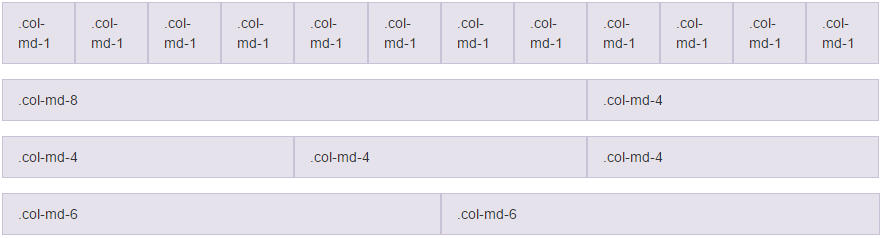
\includegraphics[scale=0.7]{img/Capture2.PNG}
	\captionsetup{format=hang}
	\caption[Beispiel Bootstrap Grid]{\label{fig:Grid}Beispiel Bootstrap Grid \cite{B}}

	\begin{lstlisting}[caption={Code für Abbuildung \ref{fig:Grid} \cite{B}}, label={lst:Database Query Core Node}]
<div class="row">
  <div class="col-md-1">.col-md-1</div>
  <div class="col-md-1">.col-md-1</div>
  <div class="col-md-1">.col-md-1</div>
  <div class="col-md-1">.col-md-1</div>
  <div class="col-md-1">.col-md-1</div>
  <div class="col-md-1">.col-md-1</div>
  <div class="col-md-1">.col-md-1</div>
  <div class="col-md-1">.col-md-1</div>
  <div class="col-md-1">.col-md-1</div>
  <div class="col-md-1">.col-md-1</div>
  <div class="col-md-1">.col-md-1</div>
  <div class="col-md-1">.col-md-1</div>
</div>
<div class="row">
  <div class="col-md-8">.col-md-8</div>
  <div class="col-md-4">.col-md-4</div>
</div>
<div class="row">
  <div class="col-md-4">.col-md-4</div>
  <div class="col-md-4">.col-md-4</div>
  <div class="col-md-4">.col-md-4</div>
</div>
<div class="row">
  <div class="col-md-6">.col-md-6</div>
  <div class="col-md-6">.col-md-6</div>
</div>
\end{lstlisting}
\end{figure}

\subsection{Landingpage (index.html)}

Die Landigpage \textit{index.html} beinhaltet größtenteils das Registrierungs- und Anmeldeformular. Die Login sowie die Registrierung sind beide durch einen Button erreichbar der ein Standard Bootstrap Modal öffnet. Dieses ist durch zwei Tabs geteilt in den Login und die Registrierun. Für die Registrierung wird lediglich der Name des zu führenden Unternehmens benötigt sowie ein Password. Mit diesen Daten erfolgt auch der Anmeldeprozess, hierbei hat der Spieler die Möglichkeit durch das aktivieren einer Checkbox sich dauerhaft auf dem Server anzumelden. Neben dem Login/Registrierungsbutton der ebenso wie unser EARTHBOUND Logo auf der Seite zentriert angezeigt wird, beinhaltet die Landingpage noch eine Navbar. Diese ist am oberen Rand fixiert und transparent, ebenso wie die Buttons die sich darauf befinden. Es gibt drei links ausgerichtete Buttons für das Impressum, die Datenschutzerklärung und eine FAQ, welche auch als Art Spielanleitung angesehen werden kann. Des weiteren sind zwei rechts ausgerichtete Buttons in der Navbar. Diese sind dazu dar die Spieler anzuzeigen, welche gerade aktiv das Spiel spielen, sowie eine Highscore Liste darzustellen, welche die besten Spieler anzeigt die das Spiel bereits abgeschlossen haben. Auch die Buttons in der Navbar öffnen Modals in dem der Content angezeigt wird. Die FAQ sind speziell als Panele in einem Bootstrap-Accordion eingebunden um die Fragen möglichst übersichtlich zu halten.
Ansonsten ist die Seite im Hintergrund mit einem Video mit transparenten schwarzen Overlay versehen, welches als MP4 und WebM eingebunden ist, somit sollte das Video von jedem Browser unterstützt werden.
\begin{figure}
	\centering
	
\includegraphics[scale=0.3]{img/mock.png}
	\captionsetup{format=hang}
	\caption[Landingpage Mockup]{\label{fig:landingpage}Landingpage Mockup}
\end{figure}
\subsection{Dashboard (home.html)}
Die Seite \textit{home.html} ist die Hauptseite des Spiels, auf welcher der Spieler dauerhaft verbleibt und entsprechende Subseiten dynamisch auf die Seite geladen werden, ohne das die Seite neu geladen wird. Aufgrund dessen ist die Seite in bestimmte Bereiche unterteilt. Am linken Rand befindet sich die Sidebar mit dazugehörigen Verweisen. Es gibt jeweils Subseiten für: Dashboard, Marketing, Human Resources, Produktion, Sales, Accounts, Research und Finances. Die Sidebar ist mit einem Hintergrundbild und einem transparenten schwarzen Overlay versehen, wie auch das Video auf der Landingpage. Der aktive Link in der Sidebar wird jeweils weiß hinterlegt und mit einem kleinen Dreieck versehen. An die Sidebar anschließend ist der Header der Seite mit Navbar. Die Navbar ist am oberen Rand fixiert und beinhaltet links ausgerichtet den Namen des Unternehmens und das aktuelle Datum, sowie rechts ausgerichtet Statusanzeigen für das Sichtguthaben, die momentane Lagerauslastung und die Anzahl an Mitarbeitern die derzeit im Unternehmen beschäftigt sind. Daneben gibt es noch einen Button dem es dem Spieler ermöglicht sich vom Server abzumelden. Den Rest der Seite nimmt ein \verb!<div>! Container mit der ID \textit{content} ein. In diesen wird der Inhalt der Unterseiten geladen, welche in den nächsten Abschnitten beschrieben werden.

\subsubsection{Dasboard}
 Die erste Unterseite ist das eigentliche Dashboard des Spiels. Hier erhält der Spieler in Form von Diagrammen einen Überblick über die Lage seines Unternehmens. Dafür wird die JavaScript Bibliothek Chart.js benutzt\cite{C}. Die Bibliothek wird benutzt um Diagramme auf Basis von HTML5, CSS3 und JavaScript generieren zu können. Der Inhalt der Seite ist durch zwei Cards in zwei Hälften geteilt. Auf der linken Seite befindet sich ein Radar Chart, welches dem Spieler Informationen zu seinen aktuellen Kennzahlen zeigt, sowie die Werte der Kennzahlen aus der letzten Periode, damit der Spieler möglichst leicht die Entwicklung seines Unternehmens verfolgen kann. Auf der rechten Seite sieht der Spieler ein Bar Chart, welches für jedes abgeschlossene Jahr Aufwendungen und Erträge des Unternehmens gegenüberstellt und einen Eindruck über die Wirtschaftlichkeit des Unternehmens gibt. Des weiteren wird der Marktanteil des Unternehmens in Relation zu allen anderen Unternehmen amMarkt angezeigt, dafür wird ein Polar Area Chart verwendet.

 \subsubsection{Marketing}
 Auf der Marketingseite wird dem Spieler die Möglichkeit gegeben Marketingkampagnen für sein unternehmen zu starten. Diese Seite, wie auch alle nachfolgenden, verwendet nur eine \textit{card}. Diese ist mit dem Grid-System in zwei gleich große Spalten aufgeteilt, wobei die linke Spalte wiederum in zwei gleich große Spalten aufgeteilt ist. In der linken beiden Spalten befinden sich jeweils zwei Panele untereinander worin dem Spieler Information über alle möglichen Kapagnen gegeben wird, wie z.B. die anfallenden kosten pro Tag und die benötigte Anzahl an Mitarbeitern. Die rechte Spalte wird dazu genutzt alle aktiven Kampagnen anzuzeigen. Dafür wird ein \textit{Panel} genutzt in das für jede Kampagne ein \textit{list-group-item} einer \textit{list-group} erstellt wird. Dort ist die Art der Kampagne sowie die Gesamtkosten aufgelistet. Außerdem gibt es für jeden Eintrag ein \textit{badge} welches die noch verbleibende Laufzeit anzeigt. Zum erstellen neuer Kampagnen befindet sich ein Button in der rechten oberen Ecke der \textit{card}. Dieser öffnet ein \textit{Modal} in dem per \textit{dropdown} die Art der Kampagne ausgewählt werden kann und über ein Input Feld die Dauer den gewünschten Kampagen angegeben werden kann.

 \subsubsection{Human Resources}
 Die Seite Human Resources ermöglicht es dem Spieler die Mitarbeiter seines Unternehmens zu verwalten. Die \textit{card} ist mit dem Grid-System in zwei Spalten eingeteilt, wobei die linke Spalte doppelt so breit ist wie die rechte. In der linken Spalte ist eine Tabelle eingebunden, welche alle momentan beschäftigten Mitarbeiter im unternehmen darstellt. In der rechten spalte wird als \textit{list-group} in einem \textit{Panel} die möglichen sozialen Leistungen angezeigt, die der Spieler aktivieren und deaktivieren kann. Dafür dient dem Spieler ein Button der in jedem \textit{list-group-item} eingefügt ist. Ob eine Leistung aktiv ist oder nicht wird dem Spieler mit Hilfe eines \textit{badges} in der rechten oberen Ecke des \textit{list-group-item} angezeigt. das Einstellen von Mitarbeitern erfolgt wieder über ein \textit{Modal}. Dieses beinhaltet zwei Input Felder für die Anzahl an Mitarbeitern die man einstellen möchte und das Gehalt was den Mitarbeitern gezahlt werden soll, sowie ein \textit{dropdown}, welches genutzt wird um die entsprechende Abteilung auszuwählen, in der der Mitarbeiter beschäftigt werden soll.

\subsubsection{Produktion}
Die Verwaltung der produktionsprozesse und Lagerverwaltung erfolgt auf der Seite Produktion. Diese ist in zwei gleich Große Spalten geteilt. Auf der Linken Seite befinden sich untereinander Panele für das Warenlager Und die Produktionshallen. Hier bekommt der Spieler einen Überblick über die maximale Lagerleistung und Produktionsfläche, sowie die Auslastung in Form einer \textit{progress-bar}. Des weiteren kann der Spieler über jeweils einen Button sein Lager und seine Produktionshallen erweitern. Darunter wird beim Erstellen einer neuen Maschine ein \textit{Accordion} erstellt, welches jede Produktionsmaschine als \textit{panel-collapse} Eintrag anzeigt. In der Rechten Spalte wird ein Bootstrap \textit{Carousel} verwendet, um zwischen den verschiedenen Produktkategorien hin und her zu schalten. Dabei wird das \textit{Carousel} neben dem Bild noch mit jeweils einer Tabelle erweitert, welche dann alle Produktlinien des jeweiligen Produktes anzeigt. Produktlinien und Produktionsmaschinen lassen sich jeweils über \textit{Modals}  hinzufügen. Bei Maschinen muss jeweils das herzustellende Produkttyp und Qualitätsstufe ausgewählt werden und bei der Erstellung von Produktlinien jeweils Produkttyp, Qualitatsstufe, Menge und Laufzeit der Produktlinie.
\begin{figure}
	\centering
	
\includegraphics[scale=0.15]{img/mock2.png}
	\captionsetup{format=hang}
	\caption[Seite Produktion Mobile Mockup]{\label{fig:produktion}Seite Produktion Mobile Mockup}
\end{figure}

\subsubsection{Sales \& Accounts}
Die Seite für den Sales liefert die Möglichkeit sich auf Ausschreibungen zu bewerben und somit Deals für sein Unternehmen zu gewinnen. Dabei ist die Seite in zwei identische Spalten aufgeteilt mit jeweils einem \textit{Accordion}. In der linken Spalte sind alle Ausschreibungen als \textit{panel-collapse} Einträge gelistet werden, mit entsprechendem Vertragsschlussdatum und in der rechten Spalte alle aktiven Bewerbungen. Hier werden zusätzlich alle Bewerber auf eine Ausschreibung angezeigt, sowie die Dauer bis Ablauf der Bewerbungsfrist.
\par Die Seite Accounts besteht zum größtenteils aus einer Liste in der alle aktiven Kunden bzw. Deals eingetragen werden. Des weiteren gibt es ein kleines \textit{Panel} in dem die Anzahl der laufenden Verträge, die zu produzierende Menge an Produkten pro Monat und der Momentane Lagerbestand dargestellt wird.

\subsubsection{Research}
Die Reasearch Seite wird genutzt um Forschungen für seine Produktlinien zu starten bzw. in Verbesserungen zu investieren. Neben einem Button für das \textit{Modal} der Seite zum Starten von Forschungen, sind auf der Seite jeweils ein \textit{panel}, welches die aktiven Forschungen anzeigt, sowie alle abgeschlossenen Forschungen. Alle Einträge in den Jeweiligen \textit{panels} erfolgt als \textit{list-group-item} in einer \textit{list-group}.

\subsubsection{Finances}
Die Finances Seite dient als Kostenübersicht für den Spieler. Außerdem können Kredite aufgenommen werden. Die \textit{card} auf der Seite ist gegliedert mit \textit{tabs} welche jeweils pro Jahr hinzugefügt werden, sodass der Spieler jeweils die Kosten und Erlöse für ein Geschäftsjahr anschauen kann. Pro \textit{tab} ist die Seite in zwei Spalten geteilt. Auf der linken Seite sind ein Bilanzstand zum aktuellen Datum abgebildet und die momentane Gewinn- und Verlustrechnung. Beides sind als \textit{table} in einem \textit{panel} eingebunden. Die rechte Spalte ist um einiges kleiner und beinhaltet eine Auflistung von allen laufenden Krediten.

\subsubsection{Anmerkungen zum Frontenddesign}
Ergänzend noch einige Anmerkungen zum Frontenddesign:

\begin{itemize}
\item Aufgrund der Längenbegrenzung der Arbeit wurde nur auf Grobe Elemente in der Seitenbeschreibung eingegangen, nicht auf die genaue implementierung. Diese kann dierekt dem Code entnommen werden.
\item Neben den beschriebenen Seiten gehören noch zusätzliche Elemente zum Design des Frontends, wie z.B. Ladebildschirme, ein Overlay falls das Unternehmen pleite geht oder diverse Fehlermeldungen
\item Neben Bootstrap werden auch einige Semantic UI Elemente verwendet.
\end{itemize}
